\documentclass[paper=letter,fontsize=11pt]{scrartcl} % KOMA-article class
\usepackage[english]{babel}
\usepackage[utf8x]{inputenc}
\usepackage[protrusion=true,expansion=true]{microtype}
\usepackage{amsmath,amsfonts,amsthm}     % Math packages
\usepackage{graphicx}                    % Enable pdflatex
\usepackage[svgnames]{xcolor}            % Colors by their 'svgnames'
\usepackage{geometry}
	%\textheight=700px                    % Saving trees ;-)
%\usepackage{url}
\usepackage[colorlinks=true,
linkcolor=blue,
urlcolor=blue]{hyperref}
\usepackage{float}
\usepackage{etaremune}
\usepackage{wrapfig}
\usepackage{framed,graphicx,xcolor}
\definecolor{shadecolor}{rgb}{0.95,0.95,1}

\usepackage{attachfile}

\frenchspacing              % Better looking spacings after periods
\pagestyle{empty}           % No pagenumbers/headers/footers

%\addtolength{\voffset}{-40pt}
%\addtolength{\textheight}{20pt}

\setlength\topmargin{0pt}
\addtolength\topmargin{-\headheight}
\addtolength\topmargin{-\headsep}
\setlength\oddsidemargin{0pt}
\setlength\textwidth{\paperwidth}
\addtolength\textwidth{-2in}
\setlength\textheight{\paperheight}
%\addtolength\textheight{-3in}
\addtolength\textheight{-2in}
\usepackage{layout}

%%% Custom sectioning}{sectsty package)
%%% ------------------------------------------------------------
\usepackage{sectsty}

\sectionfont{%			            % Change font of \section command
	\usefont{OT1}{phv}{b}{n}%		% bch-b-n: CharterBT-Bold font
	\sectionrule{0pt}{0pt}{-5pt}{3pt}}

%%% Macros
%%% ------------------------------------------------------------
\newlength{\spacebox}
\settowidth{\spacebox}{8888888888}			% Box to align text
\newcommand{\sepspace}{\vspace*{1em}}		% Vertical space macro

\newcommand{\MyName}[1]{ % Name
		\Huge \usefont{OT1}{phv}{b}{n} \hfill #1
		\par \normalsize \normalfont}

\newcommand{\MySlogan}[1]{ % Slogan}{optional)
		\large \usefont{OT1}{phv}{m}{n}\hfill \textit{#1}
		\par \normalsize \normalfont}

\newcommand{\NewPart}[2]{\section*{\uppercase{#1} #2}}

\newcommand{\PersonalEntry}[2]{
		\noindent\hangindent=2em\hangafter=0 % Indentation
		\parbox{\spacebox}{        % Box to align text
		\textit{#1}}		       % Entry name}{birth, address, etc.)
		\hspace{1.5em} #2 \par}    % Entry value

\newcommand{\SkillsEntry}[2]{      % Same as \PersonalEntry
		\noindent\hangindent=2em\hangafter=0 % Indentation
		\parbox{\spacebox}{        % Box to align text
		\textit{#1}}			   % Entry name}{birth, address, etc.)
		\hspace{1.5em} #2 \par}    % Entry value

\newcommand{\EducationEntry}[4]{
		\noindent \textbf{#1} \hfill      % Study
		\colorbox{White}{%
			\parbox{10em}{%
			\hfill\color{Black}#2}} \par  % Duration
		\noindent \textit{#3} \par        % School
		\noindent\hangindent=2em\hangafter=0 \small #4 % Description
		\normalsize \par}

\newcommand{\WorkEntry}[4]{				  % Same as \EducationEntry
		\noindent \textbf{#1} \hfill      % Jobname
		\colorbox{White}{\color{White}#2} \par  % Duration
		\noindent \textit{#3} \par              % Company
		\noindent\hangindent=2em\hangafter=0 \small #4 % Description
		\normalsize \par}

\newcommand{\PaperEntry}[7]{
		\noindent #1, ``\href{#7}{#2}", \textit{#3} \textbf{#4}, #5 (#6).}


\newcommand{\ArxivEntry}[3]{
		\noindent #1, ``\href{http://arxiv.org/abs/#3}{#2}", \textit{{cond-mat/}#3}.}

\newcommand{\BookEntry}[4]{
		\noindent #1, ``\href{#3}{#4}", \textit{#3}.}

\newcommand{\FundingEntry}[5]{
        \noindent #1, ``#2", \$#3 (#4, #5).}

\newcommand{\TalkEntry}[4]{
		\noindent #1, #2, #3 #4}

\newcommand{\ThesisEntry}[5]{
		\noindent #1 -- #2 #3 ``#4" \textit{#5}}

\newcommand{\CourseEntry}[3]{
		\noindent \item{#1: \textbf{#2} \\ #3}}

%%% Begin Document
%%% ------------------------------------------------------------
\begin{document}

%\layout

% you can upload a photo and include it here...
\begin{wrapfigure}{l}{0.5\textwidth}
	\vspace*{-2em}
		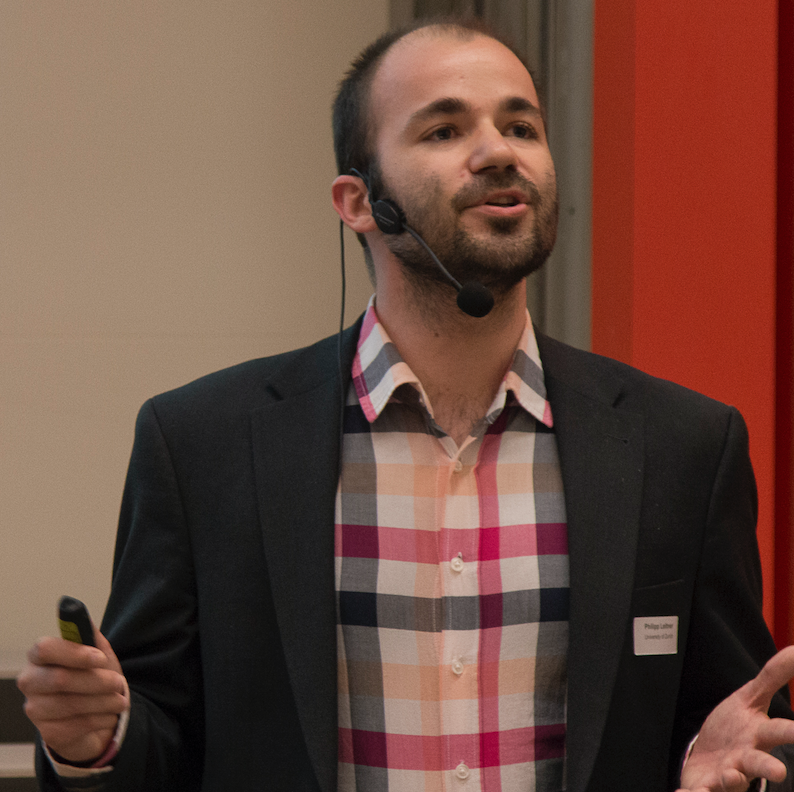
\includegraphics[width=0.18\textwidth]{profile.png}
\end{wrapfigure}

\MyName{Philipp Leitner}
\MySlogan{Curriculum Vit\ae\ (\today)}

\sepspace

%%% Personal details
%%% ------------------------------------------------------------
\NewPart{}{}

\PersonalEntry{Address}{Hörselgången 11,
  417 56 Göteborg, Sweden}
\PersonalEntry{Phone}{+41 44 63 545 81}
\PersonalEntry{Mail}{\href{mailto:philipp.leitner@chalmers.se}{philipp.leitner@chalmers.se}}
\PersonalEntry{WWW}{\href{http://philippleitner.net}{http://philippleitner.net}}

\NewPart{Summary}{}
I am currently Assistant Professor of Software Engineering at Chalmers and University of Gothenburg, Sweden, where I lead the Internet Computing and Emerging Technologies (ICET) lab. I hold a PhD degree from Vienna University of Technology (in business informatics, focussing on cost-aware service composition). My current research interests are software performance engineering, especially in a cloud computing context. My research is funded by Chalmers through the ICT Area of Advance, the Wallenberg Autonomous Systems Program (WASP), the Swiss National Science Foundation, and the European Union's 7th Framework Programme. I have published around 100 peer-reviewed publications, leading to an h-index of 27 as tracked by Google Scholar.


%%% Education
%%% ------------------------------------------------------------
\NewPart{Education}{}

\EducationEntry{PhD Business Informatics}{Oct. 2007 - Oct. 2011}{Vienna
University of Technology}{On Preventing Violations of Service Level Agreements in Composed Services using Self-Adaptation\\
Thesis advisor: Prof. Schahram Dustdar}
\sepspace

\EducationEntry{MSc Business Informatics}{Nov. 2005 - Sep. 2007}{Vienna
University of Technology}{}

\EducationEntry{BSc Business Informatics}{Oct. 2002 - Oct. 2005}{Vienna
University of Technology}{}

%%% Work experience
%%% ------------------------------------------------------------
\NewPart{Appointments and Work History}{}

\EducationEntry{Assistant Professor}{Since Aug. 17}{Chalmers $|$ University of Gothenburg}{\begin{itemize}
\item{Tenure-Track Assistant Professor}
\item{Leader of the ICET-lab}
\item{Part of the ICT Area of Advance}
\end{itemize}
}
\sepspace
\EducationEntry{Senior Research Associate}{Jan. 2014 - Jul. 2017}{University of
Zurich}{\begin{itemize}
\item{Research team leader ``cloud-based software engineering''}
\item{PI for SNF project MINCA and Co-PI for Hasler Dev-Cloud and FP7 CloudWave}
\item{Lecturer of various undergrad and graduate courses}
\end{itemize}
}
\sepspace
\EducationEntry{Postdoctoral Researcher}{Nov. 2011 - Dec. 2013}{Vienna
University of Technology}{\begin{itemize}
\item{Conducted research on cloud computing and middleware}
\item{Taught courses \emph{Advanced Internet Computing} and \emph{Distributed Systems Technologies} on graduate level}
\item{Supervised a large number of master students in their thesis work}
\end{itemize}}
\sepspace
\EducationEntry{Research and Teaching Assistant}{Oct. 2007 - Oct. 2011}{Vienna
University of Technology} {\begin{itemize}\item{Conducted research on service-based systems engineering}
\item{Taught various courses as TA}
\end{itemize}}
\EducationEntry{Research Software Engineer}{Jul. 2005 - Sep. 2007}{Siemens PSE,
Vienna}{ {\begin{itemize}\item{Worked on industrial research project in the area of telecommunications and network management}
\end{itemize}}
}
\EducationEntry{Independent Software Engineer}{2003 - 2006}{Various smaller Web projects}{}
\EducationEntry{Teaching Assistant}{2003 - 2007}{Vienna University of Technology}{}

\NewPart{Acquired Grants}{}

\begin{itemize}
  \item VR Starting Grant (2019 -- 2022), VR\\
  Sole applicant\\
	Grant value 3,639,000 SEK
  \item WASP Academic PhD Student (2017 -- 2021), WASP\\
  Main Supervisor\\
	Grant value $\approx$3,600,000 SEK
  \item Chalmers AoA Hiring Startup Package (2017 -- 2021), ICT Area of Advance\\
  Grant value 8,000,000 SEK
  \item Individual Project ``MINCA'' (2016 -- 2019), Swiss National Science Foundation\\
  Sole applicant \\
  Grant value 180,000 CHF ($\approx$1,630,000 SEK), at University of Zurich
  \item Technology Transfer Project ``DevCloud'' (2016 -- 2019), Hasler Foundation\\
  Co-applicant \\
  Grant value 50,000 CHF ($\approx$453,000 SEK), at University of Zurich
\end{itemize}

\NewPart{Research Visits}{}

  \begin{tabular}{p{12cm}l}
    Institute of of High-Performance Computing, Singapore & Feb./Mar. 2013 \\
    University of Stuttgart, Germany & Apr. 2010 \\
  \end{tabular}

% \NewPart{Past Faculty Applications}{}
%
% As requested by the SNF, I list all past faculty applications for which I
% have been invited to interviews or have been short-listed.
%
% \begin{itemize}
% \item Tenure-Track Assistant Professor at \textbf{University of Copenhagen},
% interview declined for personal reasons.
% \item Tenure-Track Assistant Professor at \textbf{Vrije Universiteit Amsterdam},
% interviewed Nov. 23rd, 2015. Ranked 2nd of 48 candidates.
% \item Tenure-Track Assistant Professor at \textbf{University of Gothenburg /
% Chalmers}, interviewed Jun. 16th, 2015. On 5-person short list of 25 candidates.
% \item Tenure-Track Research Assistant Professor at \textbf{IMDEA Madrid},
% interviewed Apr. 9th, 2013.
% \end{itemize}

\NewPart{Invited Talks and Seminars}{}

\begin{itemize}
	\item \emph{Performance stability of (public) clouds}, Invited Talk at Vehicle Electronics and Connected Services (VECS, industrial conference), scheduled for April 2019
	\item \emph{AWS Lambda and #serverless. What’s all the fuzz about?}, Invited Talk at the Chaos Engineering Days Stockholm, December 2018
		\item \emph{Software performance testing in a public cloud – how bad is it really?}, Invited Talk at the Metrics Day 2018, October 2018
		\item \emph{Performance Testing of and in the Cloud}, Invited Lecture at the IDEA League Doctoral School on Engineering Complex Systems and IT with Big data and Information Technology, September 2018
\item \emph{Predictability of Performance in Public Clouds - Some Empirical Data and Lessons Learned for Software Performance Testing}, Seminar at IBM Research, Ireland, November 2017
\item \emph{Predictability of Performance in Public Clouds - Some Empirical Data and Lessons Learned for Software Performance Testing}, Invited Talk at the Sixth International Workshop on Load Testing and Benchmarking of Software Systems (LTB 2017), co-located with ICPE'17, April 2017
\item \emph{Your User is the Canary - Practices of and Obstacles to Conducting Experiments in Production}, CHOOSE Forum, University of Zurich, September 2016
\item \emph{How Predictable is the Performance of IaaS Instances? Some Insights from Benchmarking EC2, GCE, Azure, and Softlayer}, Open Cloud Day, ZHAW Winterthur, June 2016
\item \emph{Software Development for the Cloud – Challenges and Opportunities}, Faculty of Informatics, University of Lugano, February 2016
\item \emph{Software Development for the Cloud – Challenges and Opportunities}, VU University Amsterdam, November 2015
\item \emph{Trends, Opportunities and Challenges of Software Development for the Cloud}, Indian Institute of Technology Ropar, November 2015
\item \emph{Trends, Opportunities and Challenges of Software Development for the Cloud}, Indian Institute of Technology New Delhi, November 2015
\item \emph{Software Development for the Cloud -- Challenges and Opportunities}, Chalmers, Gothenburg, June 2015
\item \emph{Engineering Java Applications for the Infrastructure-as-a-Service Cloud}, software evolution \& architecture lab, University of Zurich, Zurich, October 2013
\item \emph{Building Applications for the Infrastructure-as-a-Service Cloud with CloudScale}, IMDEA Software Institute, Madrid, April 2013
\item \emph{Building Elastic Java Applications based on CloudScale and the Infrastructure-as-a-Service Paradigm}, National University of Singapore, School of Computing, March 2013
\item \emph{Building Elastic Java Applications based on CloudScale and the Infrastructure-as-a-Service Paradigm}, University of Illinois Advanced Digital Sciences Center, Singapore, February 2013
\end{itemize}

\NewPart{Department Service}{}
\begin{itemize}
\item Postdoc Representative at the Department of Informatics, University of Zurich (2015 - 2016)
\item Member of the Habilitation Committee of Ivona Brandic (TU Vienna, 2013)
\item Member of the Habilitation Committee of Karl Michael G\"oschka (TU Vienna, 2012)
\end{itemize}

\NewPart{Professional Service}{}

\subsection*{Organized Events}
\begin{itemize}
\item Co-Organizer of the 1st \emph{Vienna Software Seminar (VSS)} on the Relation of Software Architecture and DevOps/Continuous Delivery. Organizers: Uwe Zdun, Philipp Leitner, and Florian Rosenberg.
\item Member of the Steering Committee of the International Workshop on Quality-Aware DevOps (QUDOS). From 2018.
\item Dagstuhl GI Seminar on \emph{Software Performance Engineering in the DevOps World} (September 26th – September 30th 2016, Schloss Dagstuhl, Germany). Co-organized with Andre van Hoorn, Pooyan Jamshidi, and Ingo Weber.
\item Half-day \emph{CloudWave Training Event} (September 5th 2016, TU Vienna, Austria). Half-day session at ESOCC'16. Co-organized with Andreas Metzger and Eliot Salant.
\end{itemize}

\subsection*{Editorial Memberships}
\begin{itemize}
\item Publicity Chair of Elsevier's Journal on Systems and Software (JSS). Responsible for coordinating and implementing the publicity efforts of the journal.
\item Special Issue on Converging Fog and Cloud Computing, in IEEE Cloud Computing. Co-edited with Erik Elmroth, Stefan Schulte, and Srikumar Venugopal.
\item Academic Editor of PeerJ Computer Science
\item Special Issue on Software Tools and Technologies for Monitoring and Prediction of Cloud Services, in Software: Practice and Experience (published by Wiley-Blackwell). Co-edited with Rajiv Ranjan, Raj\-kumar Buyya, Armin Haller, and Stefan Tai
\end{itemize}

\subsection*{Chairmanships}
\begin{itemize}
\item Publication Chair of 10th ACM/SPEC International Conference on Performance Engineering (ICPE)
\item PC Co-Chair of the  3rd International Workshop on Quality-Aware DevOps (QUDOS), co-located with the  8th ACM/SPEC International Conference on Performance Engineering (ICPE 2017)
\item Co-Chair of a Special Session on Services Computing and Internet Technologies (SerCo 2016) at the International Conference on High Performance Computing \& Simulation (HPCS 2016)
\item Tutorial Chair of the 16th International Conference on Web Engineering (ICWE2016)
\item Workshop Chair of the European Conference on Service-Oriented
and Cloud Computing (ESOCC) 2015.
\item General Chair of the 1st International Workshop on Monitoring and
Prediction of Cloud Services (MoPoC'12), co-located with ICSOC'12.
\end{itemize}


\subsection*{Reviews for Funding Agencies}

\begin{itemize}
  \item Natural Sciences and Engineering Research Council of Canada (NSERC)
	\item Deutscher Akademischer Austauschdienst (DAAD)
	\item Luxembourg National Research Fund (FNR)
\end{itemize}

\subsection*{Program Commitee Memberships}
\begin{itemize}
	\item IEEE International Conference on Software Analysis, Evolution and Reengineering (SANER 2019)
	\item IEEE International Conference on Software Maintenance and Evolution (ICSME 2018)
	\item International Conference on Mining Software Repositories (MSR 2018 -- 2019)
  \item ACM International Conference on Distributed Event-Based Systems (DEBS 2018)
	\item ACM/SPEC International Conference on Performance Engineering (ICPE 2018, 2020)
	\item IEEE International Conference on Cloud Computing (CLOUD, 2015 -- 2018)
	\item International Conference on the Quality of Information and Communications Technology (QUATIC, 2018)
	\item International Conference on Edge Computing (EDGE 2017)
  \item International Symposium on Fog and Edge Computing (ISFEC 2017)
	\item Euromicro Conference on Software Engineering and Advanced Applications (SEAA, 2018)
	\item International Conference on Service-Oriented Computing (ICSOC, 2015 -- 2017)
  \item European Conference on Service-Oriented and Cloud Computing (ESOCC, 2015, 2017)
  \item International Conference on Web Engineering (ICWE, 2015, 2019)
  \item IEEE/ACM International Utility and Cloud Computing Conference (UCC, 2014 -- 2017)
  \item International Conference on Service Oriented Computing and Applications (SOCA, 2014 -- ongoing)
	\item Cloud Challenge, held in conjunction with UCC (2014)
	\item International Workshop on RESTFul Designs (WS-REST, co-located with WWW, 2018)
	\item International Workshop on Software Engineering Aspects of Continuous Development and New Paradigms of Software Production and Deployment (DEVOPS, 2018)
  \item International Workshop on Autonomous Control for Performance and Reliability Trade-offs in Internet of Services (ACPROSS, 2017)
	\item International Workshop on Inter-Organizational Processes (IOPs, 2016)
    \item  International Workshop on Big Data Software Engineering (BIGDSE, 2015 -- ongoing)
  \item EAI International Conference on Cloud, Networking for IoT Systems (CN4IoT, 2015)
  \item International Conference on Internet and Web Applications and Services (ICIW, 2014 -- 2015)
  \item International Conference on the Future Internet of Things and Cloud (FiCloud, 2014)
    \item International Conference on Service Oriented Computing (ICSOC) Demonstration Track (2014 -- ongoing)
    \item International Workshop on Federative and Interoperable Cloud Infrastructures (FedICI, 2014)
    \item International Workshop on Engineering Cloud Applications \& Services (EnCASE, 2014)
  \item Central-European Workshop on Services and their Composition (ZEUS, 2012 -- ongoing)
  \item International Workshop on Evolutionary Business Processes EVL-BP), co-located with EDOC (2011 -- 2013)
  \item International Workshop on Principles of Engineering Service-Oriented Systems (PESOS), co-located with ICSE (2013)
  \item Track on Provisioning and Management of Service Oriented Architecture and Cloud Computing (PROMASC), a Track of the WETICE (2011 -- 2012)
  \item International Workshop on Performance Assessment and Auditing in Service Computing (PAASC), co-located with ICSOC (2011 -- 2012)
  \item Workshop on Emerging Web Services Technology (WEWST), co-located
  with ECOWS (2009 -- 2011)
  \item International Workshop on Dynamic and Declarative Business
  Processes (DDBP), co-located with EDOC (2010)
\end{itemize}

\subsection*{Reviews for Journals}

(partial list)

\begin{itemize}
\item IEEE Transactions on Software Engineering (TSE)
\item Springer Empirical Software Engineering (ESEM)
\item ACM Transactions on Internet Technology (TOIT)
\item IEEE Transactions on Cloud Computing (TCC)
\item Wiley Concurrency and Computation: Practice and Experience
\item Oxford Press: The Computer Journal
\item International Journal of Communication Networks and Distributed Systems (IJCNDS)
\item Elsevier Information Processing Letters (IPL)
\item IEEE Internet Computing (IC)
\item IEEE Software
\item Elsevier Journal of Parallel and Distributed Computing (JPDC)
\item ACM Transactions on the Web (TWEB)
\item Elsevier Journal of Systems and Software (JSS)
\item Springer Computing (Archives for Scientific Computing)
\item Journal of Computer Science and Technology (JCST)
\item International Journal of Cooperative Information Systems (IJCIS)
\item IEEE Transactions on Services Computing (TSC)
\item Transactions on Pattern Languages of Programming (TPLoP)
\end{itemize}


\NewPart{Teaching Activities}{}

  \subsection*{Current PhD Students}

\begin{itemize}
\item \textbf{Linda Erlenhov}  (Chalmers, testing of non-functional properties)
\item \textbf{Joel Scheuner}  (Chalmers, cloud benchmarking)
\item \textbf{Christoph Laaber} (UZH, cost-aware cloud engineering, co-supervised with Harald C. Gall)
\item \textbf{Gerald Schermann} (UHZ, continuous delivery, co-supervised with Harald C. Gall)
\end{itemize}

\subsection*{Graduated PhD Students}

\begin{itemize}
\item \textbf{J\"urgen Cito} (UZH, cloud performance engineering, co-supervised with Harald C. Gall, now Postdoc at MIT)
\end{itemize}

\subsection*{Teaching at Chalmers $|$ GU}
\begin{itemize}
  \item Data Management (DIT032) (spring 2018, $\approx$ 80 students)
\end{itemize}

\subsection*{Previous Teaching at University of Zurich}
\begin{itemize}
  \item Informatik 1 (fall 2014 -- 2016, $\approx$ 250 students)
  \item Advanced Software Engineering (spring 2014 -- 2017, 10 -- 20 students)
  \item Seminar Advanced Software Engineering (fall 2015 -- 2016, 10 -- 20 students)
  \item Master Basismodul (ongoing)
  \item Informatik-Vertiefung (ongoing)
\end{itemize}

\subsection*{Previous Teaching at TU Vienna}
\begin{itemize}
  \item VO 2.0 Verteilte Systeme (fall 2013, $\approx$ 400  students)
  \item VU 2.0 Advanced Internet Computing (fall 2008 - 2013, 140 students)
  \item VU 4.0 Distributed Systems Technologies (spring 2009 - 2013, 140 students)
  \item PR 4.0 Internet Computing Lab Work (spring 2009 - 2013)
  \item UE 2.0 Verteilte Systeme (fall 2009 - fall 2010, $\approx$ 400 students)
  \item VU 2.0 Grid Computing (spring 2008 - spring 2009, 10 students)
\end{itemize}

\subsection*{Thesis Supervision at Chalmers $|$ University of Gothenburg}

\begin{itemize}
	\item Joel Rollny: An Extensible Framework for Large-Scale Mining of Performance Microbenchmarks (master's thesis, 2018)
  \item Viktor Holmqvist and Jonathan Nilsfors: Cachematic - Automatic Invalidation in Application-Level Caching Systems (master's thesis, 2018)
\end{itemize}

\subsection*{Thesis Supervision at University of Zurich}

\emph{All co-supervised with Prof. Harald C. Gall.}

\begin{itemize}
  \item Michael Susplugas: Continuous Integration and Deployment -- Case Study in an Energy Trading Company (master's thesis, 2016)
	\item Christian Davatz: Application-aware Benchmarking of IaaS Cloud Services (master's thesis, 2016)
	\item Bj\"orn Hasselmann: Mining Performance-Relevant Code Changes from Source Code Repositories (bachelor thesis, 2016)
  \item Emanuel St\"ockli: Predicting the Costs of Code Changes in Microservice Architectures based on Runtime Feedback  (master's thesis, 2015)
  \item Ilia Rhyzhov: Performance Analysis of Virtual Machines from Two Major IaaS Providers -- Amazon Web Services (EC2) and Google Compute Engine (GCE)  (master's thesis, 2015)
  \item Christian Bosshard: Feedback Driven Development -- Bringing Runtime Metrics to the Developer  (master's thesis, 2015)
  \item Joel Scheuner: Cloud WorkBench - A Web-Based Framework for Benchmarking Public Cloud Services (bachelor thesis, 2014)
\end{itemize}

\subsection*{Master's Thesis Supervision at TU Vienna}

\emph{All co-supervised with Prof. Schahram Dustdar.}

\begin{itemize}
  \item Fritz Schrogl: Transparently Migrating Java Objects at Runtime in an Infrastructure-as-a-Service Cloud (2014)
  \item J\"urgen Cito: Statistical Methods in Web Performance (2014)
  \item Constantin-Claudiu Gavrilete: Exploiting User Behavior and Markup Structures to Improve Search Result Rankings (2013)
  \item Rene Nowak: Towards Providing Unified Access To Cloud Data Storage Services (2013)
  \item Denitsa Djamiykova: Monitoring the Correspondence of Physical and Virtual Network Resources in OpenFlow Based Software Defined Networks (2013)
  \item Johannes Ferner:  Using Time Series Analysis to Predict Service Level Agreement Violations in Service Compositions (2012)
\item Petra Bierleutgeb:  VRoxy -- Enriching SOAs With Proxy-Based Dynamic
  Binding and Reporting Based on VRESCo (joint work with mercatis information systems GmbH, 2012)
  \item Matthias Irlacher: Using Domain-specific Languages for Event-based QoS monitoring in Service-oriented Environments. (co-supervised with Ernst Oberortner, 2011)
  \item Mathias Hess:  Reducing SLA Violations of Composite Services Deployed to the Cloud (2011)
  \item Stefan Prennsch\"utz-Sch\"utzenau:  SOA Security Policy Validation and
  Authoring (work carried out at IBM T.J. Watson Research Center, New York, 2011)
    \item Anton Korosec:  Deploying a Web Service Runtime Environment into the
  Cloud (2010)
  \item Klaus Zettler:  Planung, Konzeption und Implementierung eines Virtual
  Campus im Rahmen von S-Cube (2010)
  \item Waldemar Hummer:  Towards a Domain-Specific Language for Defining
  Intra-Service Protocols of Stateful Web Services (2009)
\end{itemize}

\newpage

%%% Papers
%%% ------------------------------------------------------------

\NewPart{Academic Journal Papers}{\href{https://scholar.google.ch/citations?user=wZ9f8CAAAAAJ}{[scholar]}}

\begin{itemize}
	\item \textbf{P. Leitner}, E. Wittern, J. Spillner, and W. Hummer: \emph{A Mixed-Method Empirical Study of Function-as-a-Service Software Development in Industrial Practice}, Journal of Systems and Software, 2018. To appear.
	\begin{shaded}
		\item  G. Schermann, J. Cito, \textbf{P. Leitner}, U. Zdun, and H. Gall: \emph{We're Doing It Live: A Multi-Method Empirical Study on Continuous Experimentation}, Information and Software Technology, 2018. To appear.
		\end{shaded}
	\item  G. Schermann, J. Cito, and \textbf{P. Leitner}: \emph{Continuous Experimentation - Challenges, Implementation Techniques, and Current Research}, IEEE Software, 2018. To appear.
	\item  O. Skarlat, M. Nardelli, S. Schulte, M. Borkowski, and \textbf{P. Leitner}: \emph{Resource Provisioning for IoT Services in the Fog}, Service-Oriented Computing and Applications, Springer, 2017. To appear.
  \begin{shaded}
  \item  \textbf{P. Leitner} and J. Cito: \emph{Patterns in the Chaos -- a Study of Performance Variation and Predictability in Public IaaS Clouds}, ACM Transactions on Internet Technology (TOIT), vol. 16, iss. 3, 2016.
   \end{shaded}
   \begin{shaded}
  \item  R. Zabolotnyi, \textbf{P. Leitner}, W. Hummer, and S. Dustdar: \emph{JCloudScale: Closing the Gap Between IaaS and PaaS}, ACM Transactions on Internet Technology (TOIT),  vol. 15, iss. 3, p. 10:1–10:20, 2015.
  \end{shaded}
  \item J. Cito, D. Gotowka, \textbf{P. Leitner}, R. Pelette, D. Suljoti, and S. Dustdar: \emph{Identifying Web Performance Degradations through Synthetic and Real-User Monitoring}, Journal of Web Engineering, 2015.
  \item  A. Metzger, \textbf{P. Leitner}, D. Ivanovic, E. Schmieders, R. Franklin, M. Carro, S. Dustdar, and K. Pohl: \emph{Comparing and Combining Predictive Business Process Monitoring Techniques}, IEEE Transactions on Systems, Man, and Cybernetics: Systems, vol. 45, no. 2, pp. 276 - 290. 2014.
  \item C. Inzinger, W. Hummer, B. Satzger, \textbf{P. Leitner}, and S. Dustdar: \emph{Generic Event-Based Monitoring and Adaptation Methodology for Heterogeneous Distributed Systems}, Software: Practice and Experience, 2014.
  \item \textbf{P. Leitner}, W. Hummer and S. Dustdar: \emph{Data-Driven and Automated Prediction of Service Level Agreement Violations in Service Compositions}, Distributed and Parallel Databases (Springer), vol. 31, no. 3, pp. 447 - 470. 2013
  \item W. Hummer, O. Raz, O. Shehory, \textbf{P. Leitner}, and S. Dustdar: \emph{Testing of Data-Centric and Event-Based Dynamic Service Compositions}, Software Testing, Verification and Reliability, vol. 23, iss. 6, pp. 465-497, 2013.
  \begin{shaded}
  \item \textbf{P. Leitner}, W. Hummer and S. Dustdar: \emph{Cost-Based
  Optimization of Service Compositions}, IEEE Transactions on Services Computing (TSC). 2011, doi:10.1109/TSC.2011.53
  \end{shaded}
\item W. Hummer, \textbf{P. Leitner} and S. Dustdar: \emph{SEPL - A
Domain-Specific Language and Execution Environment for Protocols of Stateful Web
Services}, Distributed and Parallel Databases (DPD), vol. 29, nr. 4, pp.
277-307. 2011, doi:10.1007/s10619-011-7079-6
\item B. Wetzstein, \textbf{P. Leitner}, F. Rosenberg, S. Dustdar and F. Leymann: \emph{Identifying Influential Factors of Business Process Performance Using Dependency Analysis}, Enterprise Information Systems (EIS), vol. 5, nr. 1. 2011, doi:10.1080/17517575.2010.493956
  \begin{shaded}
\item A. Michlmayr, F. Rosenberg, \textbf{P. Leitner} and S. Dustdar: \emph{End-to-End Support for QoS-Aware Service Selection, Binding and Mediation in VRESCo}, IEEE Transactions on Services Computing (TSC), vol. 3, nr. 3, pp. 193-205. 2010, doi:10.1109/TSC.2010.20
  \end{shaded}
\item A. Michlmayr, F. Rosenberg, \textbf{P. Leitner} and S. Dustdar: \emph{Selective Service Provenance in the VRESCo Runtime}, International Journal on Web Services Research (JWSR), vol 7, no. 2, pp. 65-86, 2010, doi: 10.4018/jwsr.2010040104
\item \textbf{P. Leitner}, F. Rosenberg, S. Dustdar, Daios: \emph{Efficient Dynamic Web Service Invocation}, IEEE Internet Computing, vol. 13, no. 3, pp. 72-80, May/June 2009, doi:10.1109/MIC.2009.57
\end{itemize}

\NewPart{Academic Conference Papers}{\href{https://scholar.google.ch/citations?user=wZ9f8CAAAAAJ}{[scholar]}}

\begin{itemize}
		\begin{shaded}
	\item J. Cito, \textbf{P. Leitner}, M. Rinard, and H. C. Gall: \emph{Interactive Production Performance Feedback in the IDE}, in Proceedings of the 41st ACM/IEEE International Conference on Software Engineering (ICSE). 2019.
\end{shaded}
	\item V. Holmqvist, J. Nilsfors, and \textbf{P. Leitner}: \emph{Cachematic -- Automatic Invalidation in Application-Level Caching Systems}, in Proceedings of the 2019 ACM/SPEC  International Conference on Performance Engineering (ICPE) -- Industry Track. 2019.
	\item G. Schermann and \textbf{P. Leitner}: \emph{Search-Based Scheduling of Experiments in Continuous Deployment}, in Proceedings of the 34rd IEEE International Conference on Software Maintenance and Evolution (ICSME). 2018.
	\begin{shaded}
	\item C. Laaber and \textbf{P. Leitner}: \emph{An Evaluation of Open-Source Software Microbenchmark Suites for Continuous Performance Assessment}, in Proceedings of the 15th International Conference on Mining Software Repositories (MSR), 2018.
	\end{shaded}
	\item C. Vassallo, G. Schermann, F. Zampetti, D. Romano, \textbf{P. Leitner}, A. Zaidman, M. Di Penta, and S. Panichella: \emph{A Tale of CI Build Failures: an Open Source and a Financial Organization Perspective}, in Proceedings of the 33rd IEEE International Conference on Software Maintenance and Evolution (ICSME). 2017
	\item G. Mazlamo, J. Cito, and \textbf{P. Leitner}: \emph{Extraction of Microservices from Monolithic Software Architectures}, in Proceedings of the 24th IEEE International Conference on Web Services (ICWS) - Applications Track. 2017
	\item J. Cito, G. Schermann, E. Wittern, \textbf{P. Leitner}, S. Zumberi, and H. C. Gall: \emph{An Empirical Analysis of the Docker Container Ecosystem on GitHub}, in Proceedings of the 14th International Conference on Mining Software Repositories (MSR), 2017.
	\item T. Rausch, W. Hummer, \textbf{P. Leitner}, and S. Schulte: \emph{An Empirical Analysis of Build Failures in the Continuous Integration Workflows of Java-Based Open-Source Software}, in Proceedings of the 14th International Conference on Mining Software Repositories (MSR), 2017.
	\item C. Davatz, C. Inzinger, J. Scheuner, and \textbf{P. Leitner} : \emph{An Approach and Case Study of Cloud Instance Type Selection for Multi-Tier Web Applications}, in Proceedings of the 17th IEEE/ACM International Symposium on Cluster, Cloud and Grid Computing (CCGrid), 2017.
	\item J. Cito, F. Oliveira, \textbf{P. Leitner}, P. Nagpurkar, and H. C. Gall: \emph{Context-Based Analytics – Establishing Explicit Links between Runtime Traces and Source Code}, In Proceedings of the 38th International Conference on Software Engineering (ICSE'17) -- Software Engineering in Practice (SEIP) Track, 2017.
        \item \textbf{P. Leitner} and CP. Bezemer: \emph{An Exploratory Study of the State of Practice of Performance Testing in Java-Based Open Source Projects}, in  Proceedings of the 7th ACM/SPEC International Conference on Performance Engineering (ICPE), 2017.
	\begin{shaded}
	\item G. Schermann, D. Sch\"oni, \textbf{P. Leitner}, and H. C. Gall: \emph{Bifrost -- Supporting Continuous Deployment with Automated Enactment of Multi-Phase Live Testing Strategies}, in Proceedings of the 2016 ACM/IFIP/USENIX Middleware Conference. \textbf{Best Student Paper Award}.
    \end{shaded}
	\item \textbf{P. Leitner}, J. Cito, and E. St\"ockli: \emph{Modelling and Managing Deployment Costs of Microservice-Based Cloud Applications}, in Proceedings of the 9th IEEE/ACM International Conference on Utility and Cloud Computing (UCC), 2016.
  \item O. Skarlat, S. Schulte, M. Borkowski, and \textbf{P. Leitner}: \emph{Resource Provisioning for IoT Services in the Fog}, in Proceedings of the 9th IEEE International Conference on Service Oriented Computing \& Applications (SOCA), 2016.
	\item \textbf{P. Leitner} and J. Scheuner: \emph{Bursting With Possibilities -- an Empirical Study of Credit-Based Bursting Cloud Instance Types}, in Proceedings of the 8th IEEE/ACM International Conference on Utility and Cloud Computing (UCC), 2015.
  \item E. Salant, \textbf{P. Leitner}, K. Wallbom and J. Athes : \emph{A Framework for a Cost-Efficient Cloud Ecosystem}, in eChallenges e-2015 Conference, 2015.
  \item M. Brandtner, \textbf{P. Leitner}, H. C. Gall: \emph{Intent, Tests, and Release Dependencies: Pragmatic Recipes for Source Code Integration}, in Proceedings of the 15th IEEE International Working Conference on Source Code Analysis and Manipulation (SCAM), Bremen, Germany, 2015
  \item  D. Bruneo, A. Dadashi, \textbf{P. Leitner}, B. Moltchanov, F. J. N. De-Santos, A. Miron, E. Salant, A. M. Sharifloo, K. Wallbom, and C. Woods: \emph{CloudWave – Leveraging DevOps for Cloud Management and Application Development}, in Proceedings of the Fourth European Conference on Service-Oriented and Cloud Computing (ESOCC’15) – EU Projects Track, 2015.
  \begin{shaded}
      \item J. Cito, \textbf{P. Leitner}, T. Fritz, and H. C. Gall: \emph{The Making of Cloud Applications -- An Empirical Study on Software Development for the Cloud}, in Proceedings of the 10th Joint Meeting of the European Software Engineering Conference and the ACM SIGSOFT International Symposium on Foundations of Software Engineering (ESEC/FSE), New York, NY, USA, 2015.
      \end{shaded}
        \begin{shaded}
      \item J. Cito, \textbf{P. Leitner}, H. C. Gall, A. Dadashi, A. Keller, and A. Roth: \emph{Runtime Metric Meets Developer -- Building Better Cloud Applications Using Feedback}, in Proceedings of the 2015 ACM International Symposium on New Ideas, New Paradigms, and Reflections on Programming \& Software (Onward! 2015), New York, NY, USA, 2015.
        \end{shaded}
      \item R. Zabolotnyi, \textbf{P. Leitner}, S. Schulte, and S. Dustdar: \emph{SPEEDL -- A Declarative Event-Based Language for Cloud Scaling Definition}, in Proceedings of the Future of Software Engineering For and In Cloud, Visionary Track of IEEE Services, 2015.
  \item G. Schermann, M. Brandtner, S. Panichella, \textbf{P. Leitner}, and H. Gall: \emph{Discovering Loners and Phantoms in Commit and Issue Data}, in Proceedings of the 23rd IEEE International Conference
on Program Comprehension (ICPC 2015), 2015.
  \item M. Brandtner, S. C. M\"uller, \textbf{P. Leitner}, and H. Gall: \emph{SQA-Profiles: Rule-Based Activity Profiles for Continuous Integration Environments}, in Proceedings of the 22nd IEEE International Conference on Software Analysis, Evolution, and Reengineering (SANER15), 2015.
  \item J. Scheuner, \textbf{P. Leitner}, J. Cito, and H. Gall: \emph{Cloud WorkBench - Infrastructure-as-Code Based Cloud Benchmarking}, in Proceedings of the 6th IEEE International Conference on Cloud Computing Technology and Science (CloudCom14), 2014.
  \item J. Cito, D. Suljoti, \textbf{P. Leitner}, and S. Dustdar: \emph{Identifying Root Causes of Web Performance Degradation using Changepoint Analysis}, in Proceedings of the 14th International Conference on Web Engineering (ICWE 2014), 2014.
 \item R. Zabolotnyi, \textbf{P. Leitner}, and S. Dustdar: \emph{Profiling-Based Task Scheduling for Factory-Worker Applications in Infrastructure-as-a-Service Clouds}, in Proceedings of the 40th Euromicro Conference on Software Engineering and Advanced Applications (SEAA), 2014.
 \item A. H. Borhani, \textbf{P. Leitner}, B. Lee, X. Li, and T. Hung: \emph{WPress: Benchmarking Infrastructure-as-a-Service Cloud Computing Systems for On-line Transaction Processing Applications}, in Proceedings of the 18th IEEE International Enterprise Distributed Object Computing Conference (EDOC), 2014.
\item C. Inzinger, W. Hummer, I. Lytra, \textbf{P. Leitner}, H. Tran, U. Zdun and S. Dustdar: \emph{Decisions, Models, and Monitoring - A Lifecycle Model for the Evolution of Service-Based Systems}, to appear at the 17th IEEE International Enterprise Computing Conference (EDOC'13), 2013
\item C. Inzinger, B. Satzger, \textbf{P. Leitner}, W. Hummer, and S. Dustdar:
\emph{Position Paper: Model-based Adaptation of Cloud Computing Applications},  in: Proceedings of the International Conference on Model-Driven Engineering and Software Development (MODELSWARD), Special Track on Model-driven Software Adaptation (MODA), 2013
\item C. Inzinger, W. Hummer, B. Satzger, \textbf{P. Leitner}, and S. Dustdar:
\emph{Identifying Incompatible Service Implementations using Pooled Decision Trees},  in: Proceedings of the 28th Symposium on Applied Computing (SAC), Track on Dependable and Adaptive Distributed Systems, 2013
\item \textbf{P. Leitner}, C. Inzinger, W. Hummer, B. Satzger, and S. Dustdar:
\emph{Application-Level Performance Monitoring of Cloud Services Based on the Complex Event Processing Paradigm}, in: Proceedings of the 2012 IEEE International Conference on Service-Oriented Computing and Applications (SOCA'12), 2012
  \begin{shaded}
\item W. Hummer, B. Satzger, \textbf{P. Leitner}, C. Inzinger and S. Dustdar:
\emph{Deriving a Unified Fault Taxonomy for Distributed Event-Based Systems}, in: Proceedings of the 6th ACM International Conference on Distributed Event-Based Systems (DEBS), 2012
  \end{shaded}
\item \textbf{P. Leitner}, W. Hummer, B. Satzger, C. Inzinger and S. Dustdar:
\emph{Cost-Efficient and Application SLA-Aware Client Side Request Scheduling in an Infrastructure-as-a-Service Cloud}, in: Proceedings of the IEEE International Conference on Cloud Computing (CLOUD'12), 2012
\item \textbf{P. Leitner}, B. Satzger, C. Inzinger, W. Hummer and S. Dustdar:
\emph{CloudScale -- a Novel Middleware for Building Transparently Scaling
Cloud Applications}, in: Proceedings of the 27th Symposium On Applied Computing (SAC),
Track on Cloud Computing, 2012
\item C. Inzinger, B. Satzger, W. Hummer, \textbf{P. Leitner} and S. Dustdar:
\emph{Non-Intrusive Policy Optimization for Dependable and Adaptive Service-Oriented Systems}, in: Proceedings of the 27th Symposium On Applied Computing (SAC),
Track on Dependable and Adaptive Distributed Systems, 2012
\item \textbf{P. Leitner}, W. Hummer, B. Satzger and S. Dustdar:
\emph{Stepwise and Asynchronous Runtime Optimization of Web Service
Compositions}, in: Proceedings of the 12th International Conference on Web
Information System Engineering (WISE'11), Short Paper Track, 2011
\item W. Hummer, B. Satzger, \textbf{P. Leitner} and S. Dustdar:
\emph{Distributed Continuous Queries Over Web Service Event Streams}, in: Proceedings of the 7th International Conference on Next Generation Web Services Practices
(NWeSP'11), 2011
\item W. Hummer, \textbf{P. Leitner}, B. Satzger and S. Dustdar:
\emph{Dynamic Migration of Processing Elements for Optimized Query Execution in
Event-based Systems}, in: Proceedings of the International Symposium on Distributed
Objects, Middleware, and Applications (DOA 2011), 2011
\item B. Satzger, W. Hummer, \textbf{P. Leitner} and S. Dustdar:
\emph{Esc: Towards an Elastic Stream Computing Platform for the Cloud},
in: Proceedings of the 4th IEEE International Conference on Cloud Computing (CLOUD'11), Industry and Applications Track, 2011
\item W. Hummer, O. Raz, O. Shehory, \textbf{P. Leitner} and S. Dustdar:
\emph{Test Coverage of Data-Centric Dynamic Compositions in Service-Based
Systems}, in: Proceedings of the 4th International Conference on Software Testing,
Verification and Validation (ICST), 2011
\item W. Hummer, \textbf{P. Leitner} and S. Dustdar: \emph{WS-Aggregation: Distributed Aggregation of Web Services Data}, in: Proceedings of the 26th Symposium On Applied Computing (SAC), Track on Service-Oriented Architectures and Programming , 2011
  \begin{shaded}
\item \textbf{P. Leitner}, B. Wetzstein, D. Karastoyanova, W. Hummer, S. Dustdar and F. Leymann: \emph{Preventing SLA Violations in Service Compositions Using Aspect-Based Fragment Substitution}, in: Proceedings of the International Conference on Service-Oriented Computing (ICSOC) , 2010
  \end{shaded}
\item \textbf{P. Leitner}, A. Michlmayr, F. Rosenberg and S. Dustdar: \emph{Monitoring, Prediction and Prevention of SLA Violations in Composite Services}, in: Proceedings of the IEEE International Conference on Web Services (ICWS), Industry and Applications Track, 2010
\item F. Rosenberg, M. B. M\"uller, \textbf{P. Leitner}, A. Michlmayr, A. Bouguettaya
and S. Dustdar: \emph{Metaheuristic Optimization of Large-Scale QoS-Aware Service Compositions}, in: Proceedings of the IEEE International Services Computing Conference (SCC), 2010
\item \textbf{P. Leitner}, A. Michlmayr, F. Rosenberg and S. Dustdar: \emph{Selecting Web Services Based on Past User Experiences}, in: Proceedings of the 2009 Asia-Pacific Services Computing Conference (APSCC 2009), 2009
\item B. Wetzstein, \textbf{P. Leitner}, F. Rosenberg, I. Brandic, F. Leymann and S. Dustdar: \emph{Monitoring and Analyzing Influential Factors of Business Process Performance}, in: Proceedings of the IEEE International Enterprise Computing Conference (EDOC), 2009
\item F. Rosenberg, P. Celikovic, A. Michlmayr, \textbf{P. Leitner} and S. Dustdar: \emph{An End-to-End Approach for QoS-Aware Service Composition}, in: Proceedings of the IEEE International Enterprise Computing Conference (EDOC), 2009
\item \textbf{P. Leitner}, A. Michlmayr, F. Rosenberg, S. Dustdar: \emph{End-to-End Versioning Support for Web Services}, in: Proceedings of the IEEE Services Computing Conference (SCC), 2008
\item A. Michlmayr, F. Rosenberg, \textbf{P. Leitner} and S. Dustdar: \emph{QoS-Aware Service Provenance in Web Service Runtimes}, in: Proceedings of the IEEE International Conference on Web Services (ICWS), 2009
\item A. Michlmayr, F. Rosenberg, \textbf{P. Leitner} and S. Dustdar: \emph{Advanced Event Processing and Notifications in Service Runtime Environments}, in: Proceedings of the IEEE International Conference on Distributed Event-Based Systems (DEBS), 2008
\item R. Marin, J. Vivero, \textbf{P. Leitner}, A. Neppach and M. Zach: \emph{Securing the Madeira Network Management System}, in: Proceedings of the IEEE International Conference on Software, Telecommunications and Computer Networks (SoftCom), 2007
\item M. Leitner, \textbf{P. Leitner}, M. Zach, S. Collins and C. Fahy: \emph{Fault
Management Based on Peer-to-Peer Paradigms; A Case Study Report from the CELTIC
Project Madeira}, in: Proceedings of the IFIP/IEEE International Symposium on Integrated
Management (IM), 2007
\item R. Marin, J. Vivero, H. Nguyen, J. Serrat, \textbf{P. Leitner}, M. Zach and C. Fahy: \emph{A Distributed Policy Based Solution in a Fault Management Scenario}, in: Proceedings of the IEEE Global Communications Conference (GLOBECOM), Short Paper Track, 2006
\end{itemize}

\NewPart{Workshop, Poster, Short Paper, and Demo Contributions}{\href{https://scholar.google.ch/citations?user=wZ9f8CAAAAAJ}{[scholar]}}

\begin{itemize}
	\item J. Cito, \textbf{P. Leitner}, C. Bosshard, M. Knecht, G. Mazlami, and H. Gall: \emph{PerformanceHat - Augmenting Source Code with Runtime Performance Traces in the IDE}, in Proceedings of the 40th International Conference on Software Engineering (ICSE) - Companion Volume (Demo Track), 2018.
	\item J. Scheuner and \textbf{P. Leitner}: \emph{A Cloud Benchmark Suite Combining Micro and Applications Benchmarks}, in Proceedings of the 4th International Workshop on Quality-Aware DevOps (QUDOS 2018), 2018.
	\item C. Laaber and \textbf{P. Leitner}: \emph{ (h $|$ g)opper: Performance History Mining and Analysis},  in Proceedings of the 7th ACM/SPEC International Conference on Performance Engineering (ICPE) -- Poster and Demonstration Track, 2017.
	\item G. Schermann, J. Cito, \textbf{P. Leitner}, and H. C. Gall: \emph{Towards Quality Gates in Continuous Delivery and Deployment}, in Proceedings of the 24TH IEEE International Conference on Program Comprehension (ICPC) – Short Paper Track, 2016. \textbf{Best Short Paper Award}
	\item J. Cito, G. Mazlami, and \textbf{P. Leitner}: \emph{TemPerf: Temporal Correlation between Performance Metrics and Source Code}, in Proceedings of the 2nd International Workshop on Quality-Aware DevOps (QUDOS 2016), 2016.
    \item G. Schermann, J. Cito, and \textbf{P. Leitner}: \emph{All the Services Large and Micro: Revisiting Industrial Practice in Services Computing}, in Proceedings of the 11th International Workshop on Engineering Service Oriented Applications (WESOA’15), co-located with ICSOC 2015, 2015.
    \item M. Brandtner, \textbf{P. Leitner}, and H. Gall: \emph{Profile-based View Composition in Development Dashboards}, in Proceedings of the 17th Workshop Software-Reengineering \& Evolution (WSRE), 2015.
  \item J. Scheuner, J. Cito, \textbf{P. Leitner}, and H. Gall: \emph{Cloud WorkBench: Benchmarking IaaS Providers based on Infrastructure-as-Code}, in Proceedings of the 24th International World Wide Web Conference (WWW'15) - Demo Track, 2015.
 \item D. Bruneo, T. Fritz, S. Keidar-Barner, \textbf{P. Leitner}, F. Longo, C. Marquezan, A. Metzger, K. Pohl, A. Puliafito, D. Raz, A. Roth, E. Salant, I. Segall, M. Villari, Y. Wolfsthal, and C. Woods: \emph{CloudWave: where Adaptive Cloud Management Meets DevOps}, in Proceedings of the Fourth International Workshop on Management of Cloud Systems (MoCS 2014), 2014.
 \item \textbf{P. Leitner}, S. Schulte, S. Dustdar, I. Pill, M. Schulz and F. Wotawa: \emph{The Dark Side of SOA Testing - Towards Testing Contemporary SOAs Based on Criticality Metrics}, in: Proceedings of the 5th International Workshop on Principles of Engineering Service-Oriented Systems (PESOS), co-located with ICSE 2013, 2013
\item R. Zabolotnyi, \textbf{P. Leitner} and S. Dustdar: \emph{Dynamic Program Code Distribution in Infrastructure-as-a-Service Clouds}, in: Proceedings of the 5th International Workshop on Principles of Engineering Service-Oriented Systems (PESOS), co-located with ICSE 2013, 2013
\item F. Wotawa, M. Schulz, I. Pill, S. Jehan, \textbf{P. Leitner}, W. Hummer, S. Schulte, P. Hoenisch and S. Dustdar: \emph{Fifty Shades of Grey in SOA Testing (Position Paper)}, in: Proceedings of the 9th Workshop on Advances in Model Based Testing (A-MOST), co-located with ICST 2013, 2013
\item C. Inzinger, W. Hummer, B. Satzger, \textbf{P. Leitner}, and S. Dustdar:
\emph{Towards Identifying Root Causes of Faults in Service-Based Applications}, in: Proceedings of the 31st IEEE International Symposium on Reliable Distributed Systems (SRDS 2012), Poster Track, 2012
\item \textbf{P. Leitner}, W. Hummer and S. Dustdar:
\emph{A Monitoring Data Set for Evaluating QoS-Aware Service-Based Systems}, in: Proceedings of the 4th International Workshop on Principles of Engineering Service-Oriented Systems (PESOS), co-located with ICSE'12, 2012
\item \textbf{P. Leitner}, F. M. Nardini, G. Tolomei, F. Silvestri
and S. Dustdar: \emph{Mining Lifecycle Event Logs for Enhancing
Service-based Applications}, in: Proceedings of the 1st International Workshop on Adaptive Services
for the Future Internet (WAS4FI), colocated with ServiceWave'11, 2011
\item W. Hummer, \textbf{P. Leitner} and S. Dustdar: \emph{A Step-By-Step Debugging Technique To Facilitate Mashup Development and Maintenance}, in: Proceedings of the 4th International Workshop on Web APIs and Services Mashups (Mashups'10) co-located with ECOWS 2010, 2010
\item \textbf{P. Leitner}, B. Wetzstein, F. Rosenberg, A. Michlmayr, S. Dustdar and F. Leymann: \emph{Runtime Prediction of Service Level Agreement Violations for Composite Services}, in: Proceedings of the 3rd Workshop on Non-Functional Properties and SLA Management in Service-Oriented Computing (NFPSLAM'09), co-located with ICSOC 2009, 2009
\item A. Michlmayr, F. Rosenberg, \textbf{P. Leitner} and S. Dustdar: \emph{Comprehensive QoS Monitoring of Web Services and Event-Based SLA Violation Detection}, in: Proceedings of the 4th International Workshop on Middleware for Service Oriented Computing (MW4SOC), co-located with MIDDLEWARE'09, 2009
\item I. Brandic, D. Music, \textbf{P. Leitner}, S. Dustdar: \emph{VieSLAF Framework: Enabling Adaptive and Versatile SLA-Management}, in: Proceedings of the 6th International Workshop on Grid Economics and Business Models (Gencon), co-located with Euro-Par'09, 2009
\item F. Rosenberg, \textbf{P. Leitner}, A. Michlmayr, P. Celikovic and S. Dustdar: \emph{Towards Composition as a Service - A Quality of Service Driven Approach}, in: Proceedings of the 1st Workshop on Information and Software as Service (WISS), co-located with ICDE'09, 2009
\item \textbf{P. Leitner}, A. Michlmayr and S. Dustdar: \emph{Towards Flexible Interface Mediation for Dynamic Service Invocations}, in: Proceedings of the 3rd Workshop on Emerging Web Services Technology (WEWST), co-located with ECOWS'08, 2008
\item F. Rosenberg, \textbf{P. Leitner}, A. Michlmayr and S. Dustdar: \emph{Integrated Metadata Support for Web Service Runtimes}, in: Proceedings of the Middleware for Web Services Workshop (MWS), co-located with EDOC'08, 2008
\end{itemize}

\NewPart{Edited Books}{\href{https://scholar.google.ch/citations?user=wZ9f8CAAAAAJ}{[scholar]}}

\begin{itemize}
	\item A. Celesti and \textbf{P. Leitner} (Eds.): \emph{Advances in
  Service-Oriented and Cloud Computing -- Workshops of ESOCC 2015, Revised Selected Papers}.
Communications in Computer and Information Science (CCIS 567). ISBN: 3319333127. 2016.

\end{itemize}

\NewPart{Contributions to Books}{\href{https://scholar.google.ch/citations?user=wZ9f8CAAAAAJ}{[scholar]}}

\begin{itemize}
	\item Rob van der Mei, Hans van den Berg, Ivan Ganchev, Kurt Tutschku, \textbf{Philipp Leitner}, Pasi Lassila, Wojciech Burakowski, Fidel Liberal, Ake Arvidsson, Tobias Hossfeld, Katarzyna Wac, Hugh Melvin, Tihana Galinac Grbac, Yoram Haddad, and Peter Key:
	\emph{State of the Art and Research Challenges in the Area of Autonomous Control for a Reliable Internet of Services},
	in: Autonomous Control for a Reliable Internet of Services, Springer, 2018.
\item W. Hummer, \textbf{P. Leitner}, A. Michlmayr, F. Rosenberg, S. Dustdar:
\emph{VRESCo -- Vienna Runtime Environment for Service-oriented Computing},
in: Service Engineering. European Research Results, Springer, 2010
\item A. Michlmayr, \textbf{P. Leitner}, F. Rosenberg and S. Dustdar: \emph{Event
Processing in Web Service Runtime Environments}, in: Handbook of
Research on Advanced Distributed Event-Based Systems, Publish/Subscribe and
Message Filtering Technologies, IGI Global, 2010
\item \textbf{P. Leitner}, F. Rosenberg, A. Michlmayr, A. Huber and S. Dustdar:
\emph{A Mediator-Based Approach to Resolving Interface Heterogeneity of Web
Services}, in: Emerging Web Services Technology, Volume 3,
Birkh\"auser, 2009
\item C. Fahy, M. Ponce de Leon, S. van der Meer, R. Marin, J. Vivero, J. Serrat,
N. Georgalas, \textbf{P. Leitner}, S. Collins and B. Baesjou: \emph{Modelling
Behaviour and Distribution for the Management of Next Generation Networks},
in Whitestein Series in Software Agent Technologies and Autonomic
Computing, Special issue on Advanced Autonomic Networking and Communication,
Birkh\"auser, 2008
\end{itemize}

\NewPart{Invited Publications and Other Non-Reviewed Material}{\href{https://scholar.google.ch/citations?user=wZ9f8CAAAAAJ}{[scholar]}}

\begin{itemize}
	\item A. van Hoorn, P. Jamshidi, \textbf{P. Leitner}, and I. Weber:
	\emph{Report from GI-Dagstuhl Seminar 16394: Software Performance Engineering in the DevOps World}, arXiv:1709.08951 [cs.PF], 2018
	\item E. Elmroth, \textbf{P. Leitner}, S. Schulte, S. Venugopal:
  \emph{Connecting Fog and Cloud Computing}, IEEE Cloud Computing, vol. 4, nr. 2, pp. 22 - 25, 2017.
	\item R. Ranjan, R. Buyya, \textbf{P. Leitner}, A. Haller, and S. Tai:
  \emph{A Note on Software Tools and Techniques for Monitoring and Prediction of Cloud Services}, Software: Practice and Experience, 2014.
  \item R. Ranjan, R. Buyya, \textbf{P. Leitner}, A. Haller, and S. Tai:
  \emph{A Note on Software Tools and Techniques for Monitoring and Prediction of Cloud Services}, Software: Practice and Experience, 2014.
  \item B. Satzger, W. Hummer, C. Inzinger, \textbf{P. Leitner}, and S. Dustdar, \emph{Winds of Change: From Vendor Lock-In to the Meta Cloud}, IEEE Internet Computing, vol. 17, no. 1, pp. 69-73, Jan.-Feb., 2013
  \item S. Tai, \textbf{P. Leitner}, S. Dustdar, \emph{Design by Units: Abstractions for Human and Compute Resources for Elastic Systems}, IEEE Internet Computing, vol. 16, no. 4, pp. 84-88, July-Aug. 2012, doi:10.1109/MIC.2012.81
  \item \textbf{P. Leitner}, S. Dustdar, B. Wetzstein, and F.
  Leymann: \emph{Cost-Based Prevention of Violations of Service Level Agreements
  in Composed Services Using Self-Adaptation}, in: Proceedings of the S-Cube@ICSE Workshop, co-located with ICSE'12, 2012
\end{itemize}

\NewPart{Theses}{\href{https://scholar.google.ch/citations?user=wZ9f8CAAAAAJ}{[scholar]}}

\begin{itemize}
  \item \textbf{P. Leitner}: \emph{On Preventing Violations of Service Level
  Agreements in Composed Services using Self-Adaptation},  PhD Thesis, Vienna
  University of Technology. Primary advisor: Prof. Schahram Dustdar. Examiner:
  Prof. Fabio Casati. 2011.
  \item \textbf{P. Leitner}: \emph{The Daios Framework -- Dynamic, Asynchronous
  and Message-oriented Invocation of Web Services},  Master's Thesis, Vienna
  University of Technology. Primary advisor: Prof. Schahram Dustdar. Responsible
  assistant: Florian Rosenberg. 2007.
\end{itemize}

\end{document}
